% !TeX root = ../../main.tex
\section{Experiments}\label{section:experiments}

Three main experiments were implemented to show how the smartphone can help with common interactions when using \ac{VR} software.
To achieve consistency amongst all experiments in terms of look and functionality, a parent class was implemented. The parent class implements multiple utilities and helpers, which are required by each experiment. It also sets up a basic scene, which contains a sky, a floor and lights.  Also the connection to the \ac{UBII} server is handled. 


\subsection{Model Viewer}\label{subsection:model-viewer}

\acl{VR} offers a new way of experiencing \ac{3D} content. It is faster to view a model from different angles and gives a feel of a real presence of the object. Model viewers like Sketchfab\footnote{Sketchfab is an online platform to public and view 3D content. Website: \href{https://sketchfab.com}{www.sketchfab.com}} implemented \ac{VR} support a while ago~\cite{AlbanDenoyel.2016}. But this experience can be enhanced with a smartphone. Models can be rotated without changing the position by walking.

\citeauthor{Katzakis.2010} implemented this without \ac{VR}. His approach uses a smartphone to rotate a model, which is displayed on a conventional display. He uses a similar setup, where the phone is wireless connected to a computer, where the model is rendered. The orientation data comes from the magnetometer and, once calibrated to the screen position, is directly mapped to the model~\cite[139]{Katzakis.2010}. In the comparison against a mouse and a touch pen, the smartphone clearly wins in terms of the time it takes to rotate to a certain pose~\cite[140]{Katzakis.2010}. 
Since this approach turned out to be very successful, it was used in this experiment. 

To feature how easy it is, to view a complex model using VR and the smartphone as a manipulator, a skeleton model is used. This experiment is the only one, supporting more than one smartphone client at the moment. For every client that connects, a new skeleton is created. The position is fixed and arranged around the position of the \ac{VR} headset. The scene is shown in Figure~\ref{fig:screenshot-exp-mv}.

\begin{figure}[htpb]
  \centering
  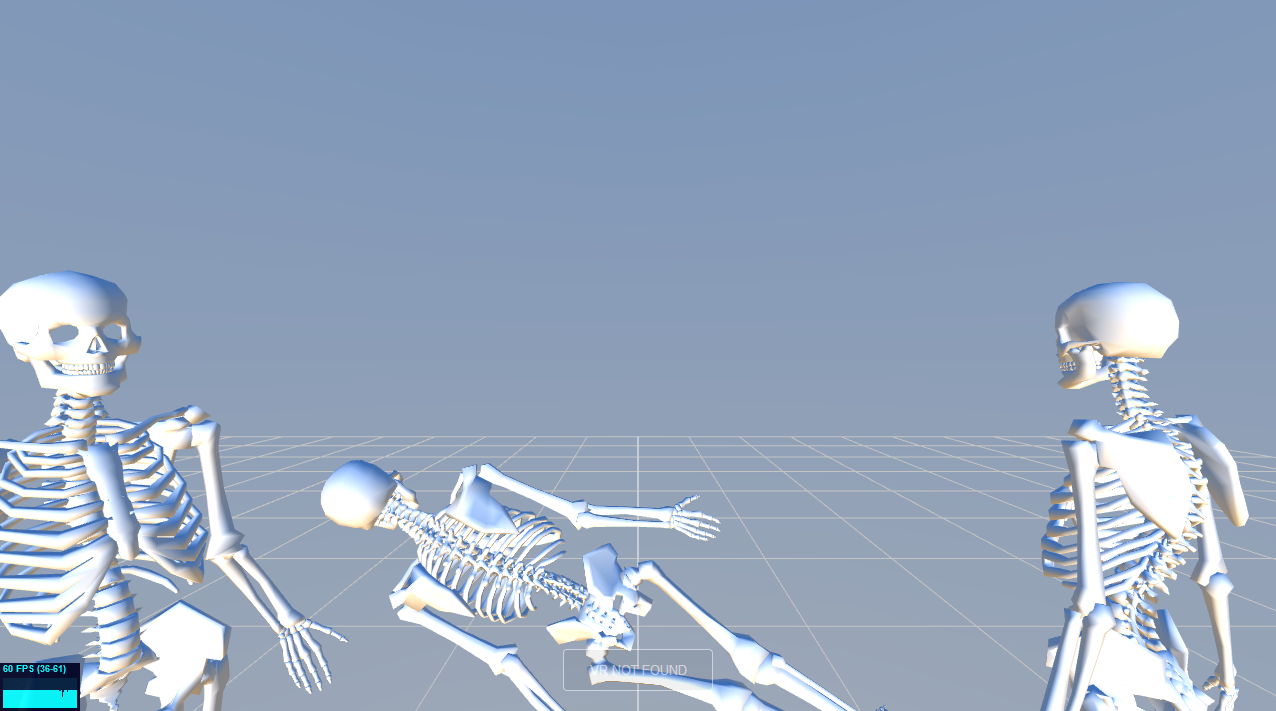
\includegraphics[width=12cm]{figures/screenshot_exp_mv.png}
  \caption[Screenshot: model viewer experiment]{A screenshot of three devices being connected and controlling the rotation of the models.}\label{fig:screenshot-exp-mv}
\end{figure}

% Note: latex thinks the hbox is overfull. This is not the case because something is fixing it. Try removing all words after the lstinline, then you will see that it overflows. But when using in an sentence it appears to be rescaled.
The implementation of this experiment listens for new clients. As soon as one connects, a new interaction is published and the resulting topic subscribed. Since the smart device publishes the orientation data in a different format than ThreeJS needs for rendering, a reusable interaction is created. The interaction converts the angles from radian to degrees, changes the coordinate system and publishes them to the \lstinline[breaklines=false]{[client id]/web-interface-smart-device/orientation}-topic. The code for the interaction is shown in Figure~\ref{fig:ubii-interaction-angles}.

\begin{figure}[H]
  \begin{lstlisting}[language=JavaScript]
    function (input, output, state) {
      if (!input) {
        return;
      }

      const deg2Rad = function(v) {
        return v * Math.PI / 180;
      };

      output.orientation = {
        x: deg2Rad(input.orientation.y),
        y: deg2Rad(input.orientation.x),
        z: deg2Rad(-input.orientation.z)
      };
    }
  \end{lstlisting}
  \caption[UBII interaction converting euler angles in radians to degrees]{This interaction is used to convert the orientation data sent by the smart device to the format ThreeJS needs for rendering. The values are converted by multiplying with the number $\Pi$ (\enquote{PI}) and dividing by $180$.}\label{fig:ubii-interaction-angles}
\end{figure}


\subsection{Laser Pointer}\label{subsection:laser-pointer}

Selecting elements in a virtual world with a \ac{VR} headset, is a basic interaction most applications need. The selection of elements in a \ac{2D} environment is no problem with standard input devices like a mouse or touch screen. But the selection in a \ac{3D} environment is problematic, because the element might be far away from the cursor or user. Raycasting is often used to solve this problem: A ray is created, with the headset or another tracked device as origin. The element first hit by the ray, is then selected. If not tracked device is present, the rotation of the headset is often used. The ray is fixed to the head of the user and casted along his viewing direction. % citation needed
This forces the user to keep the head still and look at a certain object to select it, until a button is pressed or a certain time has passed.

% explain raycasting

A better solution is the use of handheld controllers, where the position of the controller is used as origin for the ray. Since the smartphone provides orientation data, it can be used for this task, too. But most handheld controllers have also positional tracking, which allows them to represent the hand of a user. Since a smartphone does not have positional tracking, the origin has to be somewhere else. The head could be used, but then the user would have no visual representation of the rotation of the phone. A visual representation is important, so that the user can see where the ray is going, even when rotating it in the opposite direction of the view direction. To give the user a better feel for the \enquote{laser pointer} going out of his phone, a visual representation is needed. A virtual phone model is placed inside the view frustum of the user. It has a fixed position relative to the users head, so that it never leaves his view. To improve the illusion, the relative position is located where the phone could be in the real world. Similar to the first experiment (\ref{subsection:model-viewer}), the smart device position is used to adjust the rotation of the virtual phone. A line comes out of the front of the phone (the \enquote{laser}), to indicate where the ray would hit.